\subsection{Ant Colony Optimization Component Ablation}
\label{subsec:exp_ablation}

To isolate the independent contribution of each mechanism in MMAS-VND-CL, this experiment disables one mechanism at a time while keeping all other settings unchanged, yielding six groups as listed in Table~\textcolor{blue}{\ref{tab:ablation_groups}}. Each group is run 40 times on Map~1, Map~2, and kroB100. The joint evaluation remains the best cost, mean cost/standard deviation, run time, and success rate; the overall results are summarized in Table~\textcolor{blue}{\ref{tab:ablation}}. The main text retains the cost--time comparison (Fig.~\ref{fig:abl_cost_time}) as the primary visualization; more detailed convergence curves and cost distributions are moved to the accompanying experimental data document for reference when needed. The overall conclusion is as follows: VND and the MMAS pheromone bounds jointly determine whether a good solution can be obtained reliably, and neither is dispensable; pseudo-random transfer, the S-curve schedule, and the candidate list mainly govern how quickly a good solution is obtained, with relatively limited marginal effects on solution quality but decisive effects on computational cost. It should be noted in advance that some ablation groups still attain the optimal cost on individual maps, and are even faster in some cases. Such apparently better outcomes do not contradict the hierarchy above; they are explained below in terms of the underlying mechanisms.

\begin{table}[!t]
\caption{Ablation experiment groups}
\label{tab:ablation_groups}
\centering
\small
\setlength{\tabcolsep}{4pt}
\begin{tabular}{cll}
\toprule
Group & Description & Disabled Mechanism \\
\midrule
1 & Complete Algorithm & None \\
2 & No Pseudo-Random & ACS Pseudo-Random Transfer Rule \\
3 & No VND & VND Local Search \\
4 & No S-Curve & Progressive Local Search Scheduling \\
5 & No Candidate List & Candidate List Acceleration \\
6 & No MMAS & MMAS Pheromone Boundary \\
\bottomrule
\end{tabular}
\end{table}

\begin{figure}[!t]
\centering
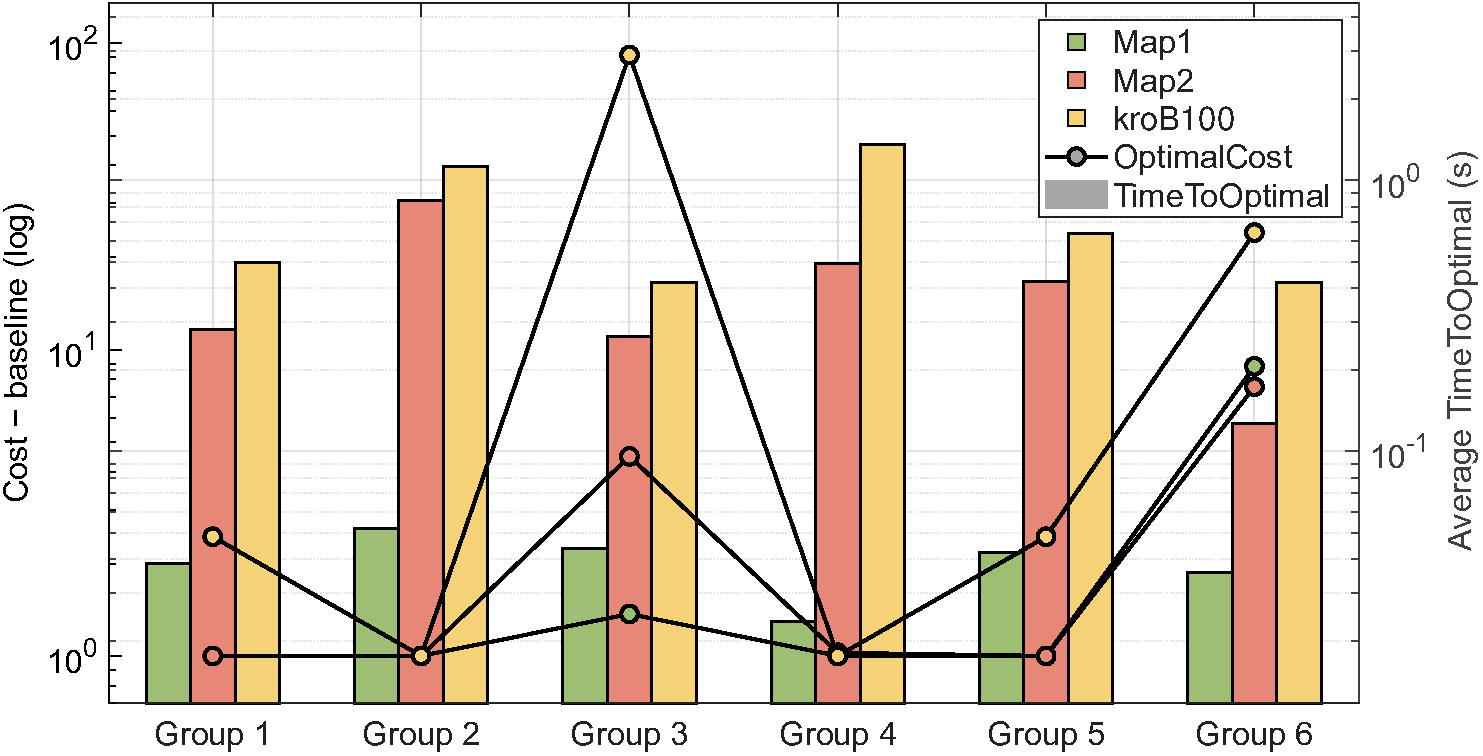
\includegraphics[width=3in]{figures/Ablation_Cost&Time}
\caption{Comparison of mean cost and mean computation time of the six ablation groups on the three maps.}
\label{fig:abl_cost_time}
\end{figure}

\begin{table}[!t]
\caption{Ablation experiment results}
\label{tab:ablation}
\centering
\footnotesize
\setlength{\tabcolsep}{2.5pt}
\begin{tabular}{cccccc}
\toprule
Map & Group & Best cost & \makecell{Path\\Mean/std.dev} & \makecell{Run Time\\(ms)} & \makecell{Success rate\\(\%)} \\
\midrule
 \multirow{6}{*}{Map 1} & 1 & \textbf{352.56} & \textbf{352.56}/\textbf{0.00} & 38.6 & \textbf{100} \\
   & 2 & \textbf{352.56} & \textbf{352.56}/\textbf{0.00} & 51.9 & \textbf{100} \\
   & 3 & \textbf{352.56} & 352.93/0.75 & 43.9 & 80 \\
   & 4 & \textbf{352.56} & \textbf{352.56}/\textbf{0.00} & \textbf{23.5} & \textbf{100} \\
   & 5 & \textbf{352.56} & \textbf{352.56}/\textbf{0.00} & 42.2 & \textbf{100} \\
   & 6 & \textbf{352.56} & 360.39/13.81 & 35.7 & 52.5 \\
\midrule
 \multirow{6}{*}{Map 2} & 1 & \textbf{623.78} & \textbf{623.78}/\textbf{0.00} & 282.9 & \textbf{100} \\
   & 2 & \textbf{623.78} & \textbf{623.78}/\textbf{0.00} & 846.4 & \textbf{100} \\
   & 3 & \textbf{623.78} & 627.26/2.53 & 265.2 & 10 \\
   & 4 & \textbf{623.78} & 623.80/0.15 & 492.9 & 97.5 \\
   & 5 & \textbf{623.78} & \textbf{623.78}/\textbf{0.00} & 422.2 & \textbf{100} \\
   & 6 & \textbf{623.78} & 630.34/6.47 & \textbf{126.8} & 10 \\
\midrule
 \multirow{6}{*}{kroB100} & 1 & \textbf{22141.00} & 22142.45/9.17 & 496.7 & 97.5 \\
   & 2 & \textbf{22141.00} & \textbf{22141.00}/\textbf{0.00} & 1126.3 & \textbf{100} \\
   & 3 & \textbf{22141.00} & 22231.50/73.36 & \textbf{419.9} & 12.5 \\
   & 4 & \textbf{22141.00} & 22141.00/0 & 1357.6 & \textbf{100} \\
   & 5 & \textbf{22141.00} & 22142.45/9.17 & 637.1 & 97.5 \\
   & 6 & \textbf{22141.00} & 22164.10/41.74 & \textbf{419.9} & 72.5 \\
\bottomrule
\end{tabular}
\end{table}

We first examine VND (Group~3). Disabling local search markedly degrades performance: the success rate on Map~2 drops to 10\%, that on kroB100 to only 12.5\%, and even Map~1 falls from 100\% to 80\%; on kroB100 the mean cost rises from 22142.45 to 22231.50 and the standard deviation expands from 9.17 to 73.36. The corresponding box plots lengthen and the convergence curves have greater difficulty reaching the optimal plateau (see the convergence curves and cost distributions in the accompanying experimental data document). This behavior is consistent with the intended mechanism: pheromone guidance during construction can only yield a reasonably ordered tour, whereas the VND composed of 2-opt, relocation, and swap is the key refinement step that drives the tour toward a local or even global optimum. Without it, the population merely wanders around coarser solutions, and both the failure rate and the variance rise accordingly.

The second component is the MMAS pheromone boundary (Group~6). Removing the dynamic $\tau_{\min}$/$\tau_{\max}$ clipping reduces the success rates on Map~1 and Map~2 to 52.5\% and 10\%, respectively, and that on kroB100 to 72.5\%, while both the mean cost and the standard deviation deteriorate noticeably. The reason is that, without boundary constraints, pheromone on early favored edges can grow without limit, the search quickly locks onto a few path structures, and typical premature convergence occurs; multiple runs fall into different suboptimal basins, hence the pattern of occasionally touching the optimum but failing in most trials. A noteworthy exception is that Group~6 is not slow on any of the three maps, and is even the fastest on Map~2. This does not indicate a faster algorithm; rather, premature homogenization of the population triggers the adaptive stopping criterion earlier and reduces ineffective iterations, trading reliability for an apparent speed advantage.

We next consider the two components that primarily affect efficiency. Removing pseudo-random transfer (Group~2) leaves the success rate on all three maps no lower than that of the complete algorithm, but the run time rises to nearly two to three times that of the full method. This shows that the value of controlled greediness lies in accelerating convergence and saving the search budget, corroborating the observation in Section~\textcolor{blue}{\ref{subsec:exp_sens}} that a lower $q_0$ is more stable but slower. Removing the S-curve schedule (Group~4), i.e., applying local search at the maximum intensity from the first iteration, still yields a 100\% success rate on kroB100, but the run time increases by about 1.7$\times$; on Map~1 the run time is in fact the shortest. These results suggest that fixed high-intensity local search need not be disadvantageous on small instances, but can rapidly exhaust the computational budget on medium and large ones. The S-curve schedule defers refinement to the second half of the iteration precisely to balance early exploration against late-stage refinement. Removing the candidate list (Group~5) leaves solution quality almost unchanged while increasing the run time, consistent with its design goal of preserving neighborhood optimality while merely reducing ineffective evaluations.

In summary, VND determines whether the optimum can be approached reliably, and the MMAS boundary determines whether the population locks in prematurely; together they form the two pillars of solution quality. Pseudo-random transfer, the S-curve schedule, and the candidate list mainly regulate the convergence rate and computational overhead. The complete algorithm attains a 100\% hit rate on Map~1 and Map~2, and a 97.5\% success rate with small variance on kroB100 in about 500~ms, representing a balanced operating point in quality, stability, and time. All subsequent algorithm comparison experiments therefore adopt the complete configuration of Group~1. If an application places greater weight on absolute success rate, the proportion of late-stage local search can be increased or the stagnation limit extended.

\subsection{Multi-Goal Traversal Comparison of Different TSP Solvers}
\label{subsec:exp_cmp}

\begin{table}[!t]
\caption{Parameter settings of the compared TSP solvers}
\label{tab:tsp_params}
\centering
\scriptsize
\begin{tabular}{>{\centering\arraybackslash}m{0.22\columnwidth} m{0.68\columnwidth}}
\toprule
Algorithm & Main parameters \\
\midrule
MMAS-VND-CL & $n_{\mathrm{ants}}=40$;
$\alpha=1$;
$\beta=2$;\newline
$\rho=0.25$;
$Q=225$;
$\tau_0=0.1$;\newline
$q_0=0.45$;
$y_{\max}=0.4$;\newline
$r_{\mathrm{elite}}=0.7$;
$k=9$ \newline
Local search transition interval$=[0,30]$;\\
\midrule
ACO & $n_{\mathrm{ants}}=40$;
$\alpha=1$;
$\beta=2$;
$\rho=0.25$;\newline
$Q=225$;
$\tau_0=0.1$;
$\mathrm{Iter}=100$ \\
\midrule
GA & $\mathrm{Pop}=100$;
$\mathrm{Iter}=1500$;\newline
$P_c=0.8$;
$P_m=0.25$;\newline
Number of elites$=10$ \\
\midrule
SA & $T_0=150$;
$\alpha=0.996$;\newline
$L=10$;
$T_{\mathrm{end}}=10^{-8}$ \\
\bottomrule
\end{tabular}
\end{table}

\begin{table}[!t]
\caption{Multi-goal traversal comparison results}
\label{tab:tsp_cmp}
\centering
\scriptsize
\setlength{\tabcolsep}{2.5pt}
\begin{tabular}{cccccc}
\toprule
Map & Algorithm & Best cost & \makecell{Path\\Mean/std.dev} & \makecell{Run Time\\(ms)} & \makecell{Success rate\\(\%)} \\
\midrule
 \multirow{4}{*}{Map 1} & MMAS-VND-CL & \textbf{352.56} & \textbf{352.56}/\textbf{0.00} & \textbf{38.6} & \textbf{100} \\
   & ACO & 361.41 & 391.53/18.44 & 90.6 & 0 \\
   & GA & 411.07 & 496.28/46.93 & 4181.1 & 0 \\
   & SA & 365.13 & 413.82/25.83 & 784.6 & 0 \\
\midrule
 \multirow{4}{*}{Map 2} & MMAS-VND-CL & \textbf{623.78} & \textbf{623.78}/\textbf{0.00} & 241.5 & \textbf{100} \\
   & ACO & 641.09 & 691.64/18.61 & \textbf{223.2} & 0 \\
   & GA & 710.83 & 868.79/66.45 & 6693.6 & 0 \\
   & SA & 655.71 & 687.25/13.02 & 506.3 & 0 \\
\midrule
 \multirow{4}{*}{kroB100} & MMAS-VND-CL & \textbf{22141.00} & \textbf{22142.45}/\textbf{9.17} & \textbf{496.7} & \textbf{97.5} \\
   & ACO & 23153.00 & 24546.05/606.87 & 534.1 & 0 \\
   & GA & 32243.00 & 36772.55/2894.73 & 8817.2 & 0 \\
   & SA & 23487.00 & 24871.05/753.20 & 516.5 & 0 \\
\bottomrule
\end{tabular}
\end{table}

With the front-end improved A* cost matrix and the virtual-node open encoding held fixed, this experiment replaces only the back-end TSP solver so as to examine the practical contribution of the sequencing module within the complete multi-goal traversal framework. Four solvers are compared: the proposed MMAS-VND-CL, a standard ant colony system (ACO), a genetic algorithm (GA), and simulated annealing (SA), with parameters given in Table~\textcolor{blue}{\ref{tab:tsp_params}}. Each combination is independently run 40 times on Map~1, Map~2, and kroB100. The conclusions can be summarized as follows: under the unified geometric cost interface and the tested parameter configurations, MMAS-VND-CL outperforms the three baseline metaheuristic implementations in solution quality, success rate, and stability, and its run time is also low in most settings. Only the lightweight ACO is slightly faster on Map~2, albeit with a clear gap in cost quality, whereas GA is clearly inferior in both quality and time. We elaborate below by metric--condition--mechanism, and discuss the individual cases that are faster but not better.

\begin{figure*}[!htbp]
\centering
\subfloat[Map~1]{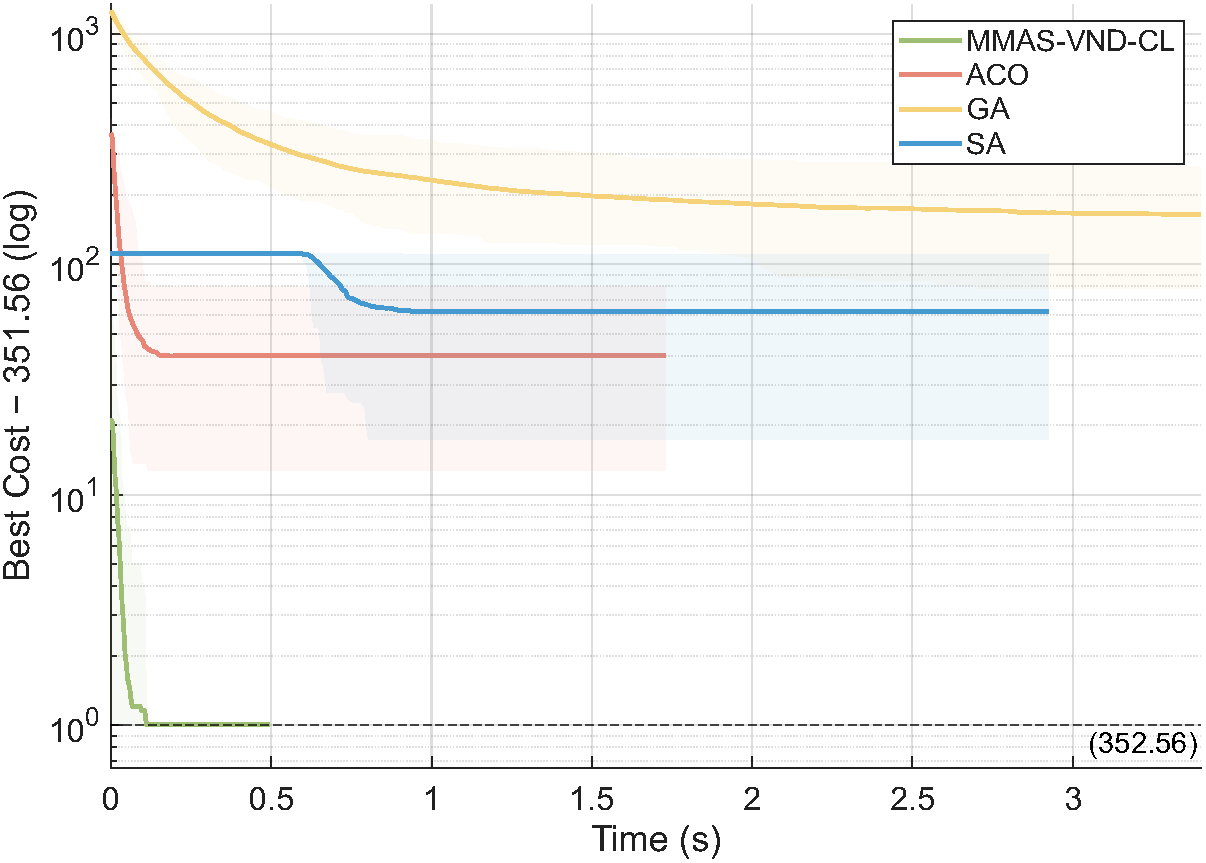
\includegraphics[width=0.3\textwidth]{figures/DifTSP_Map1_conv}}\hfil
\subfloat[Map~2]{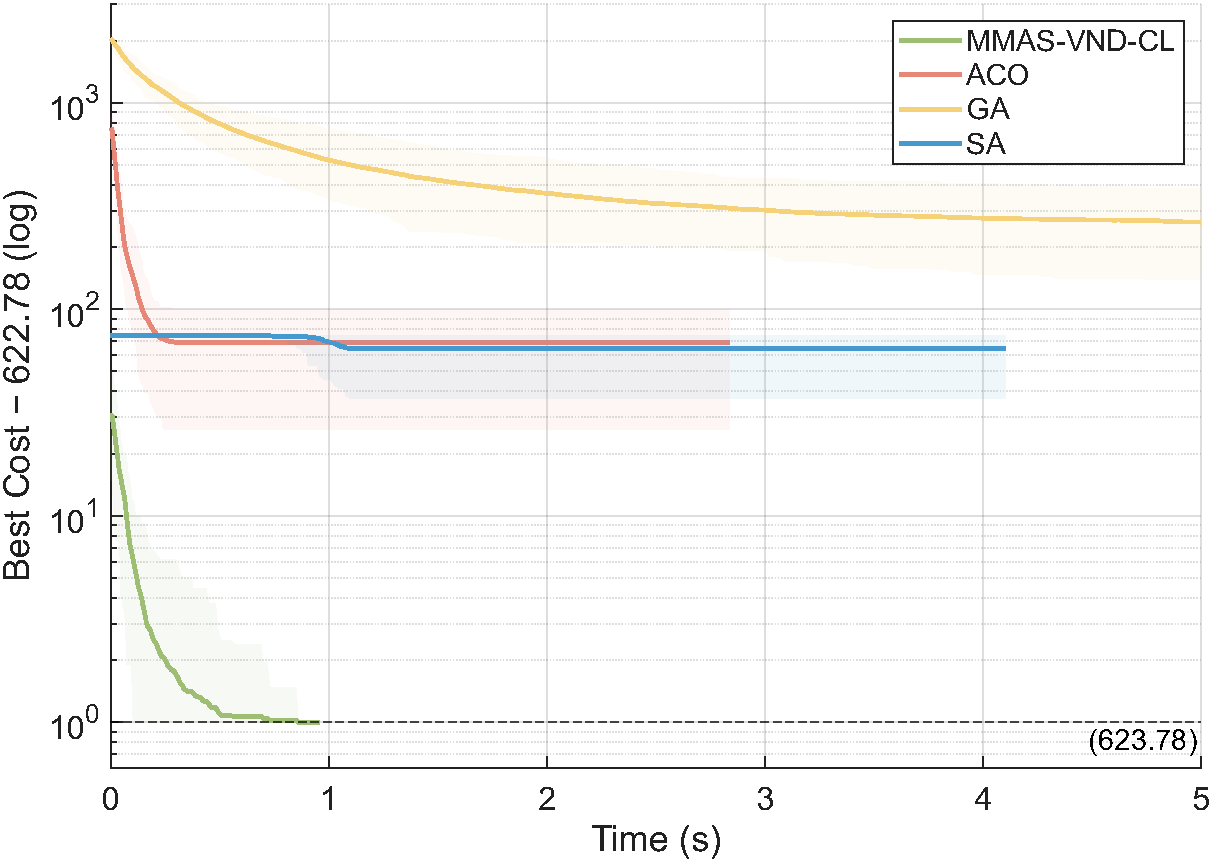
\includegraphics[width=0.3\textwidth]{figures/DifTSP_Map2_conv}}\hfil
\subfloat[kroB100]{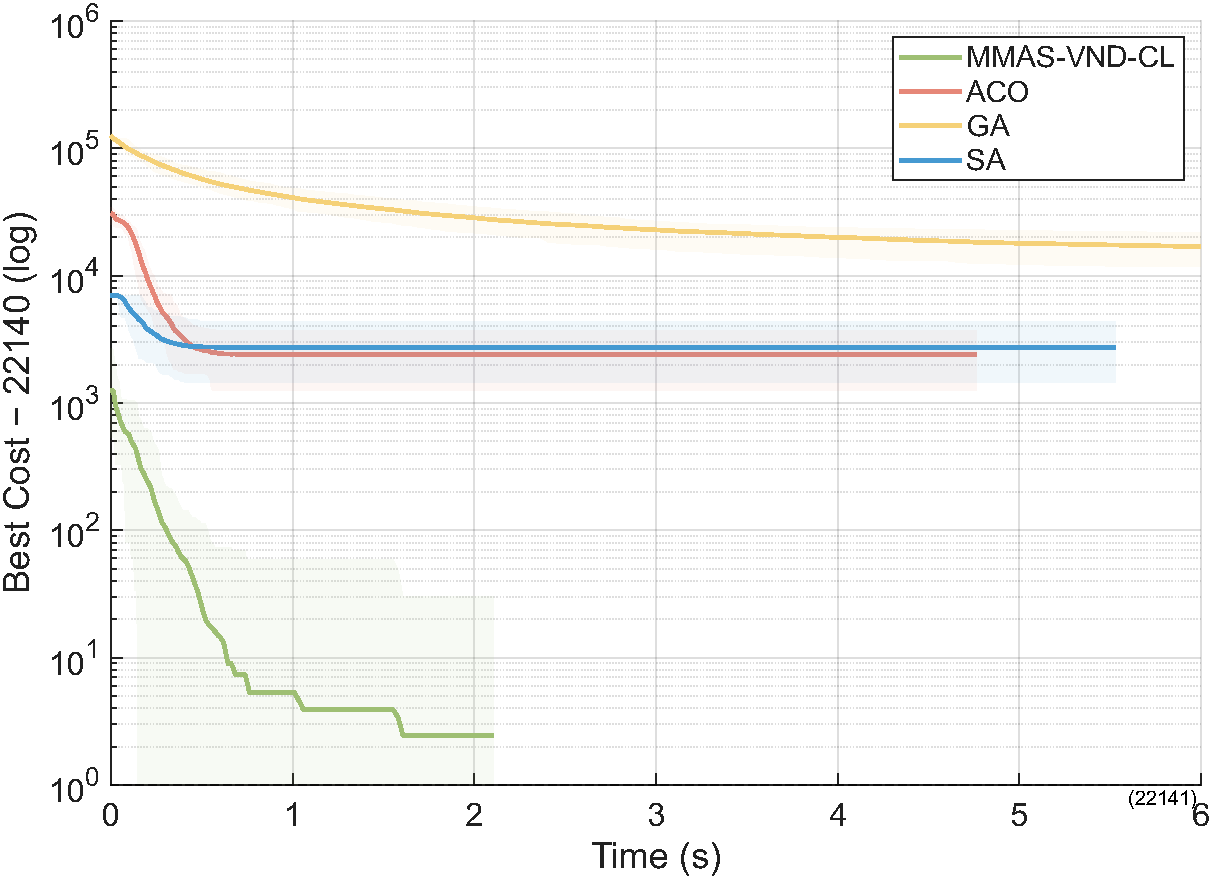
\includegraphics[width=0.3\textwidth]{figures/DifTSP_kroB100_conv}}
\caption{Mean time--cost convergence curves of the four TSP solvers over 40 runs on the three maps.}
\label{fig:tsp_conv}
\end{figure*}

\begin{figure*}[!htbp]
\centering
\subfloat[Map~1]{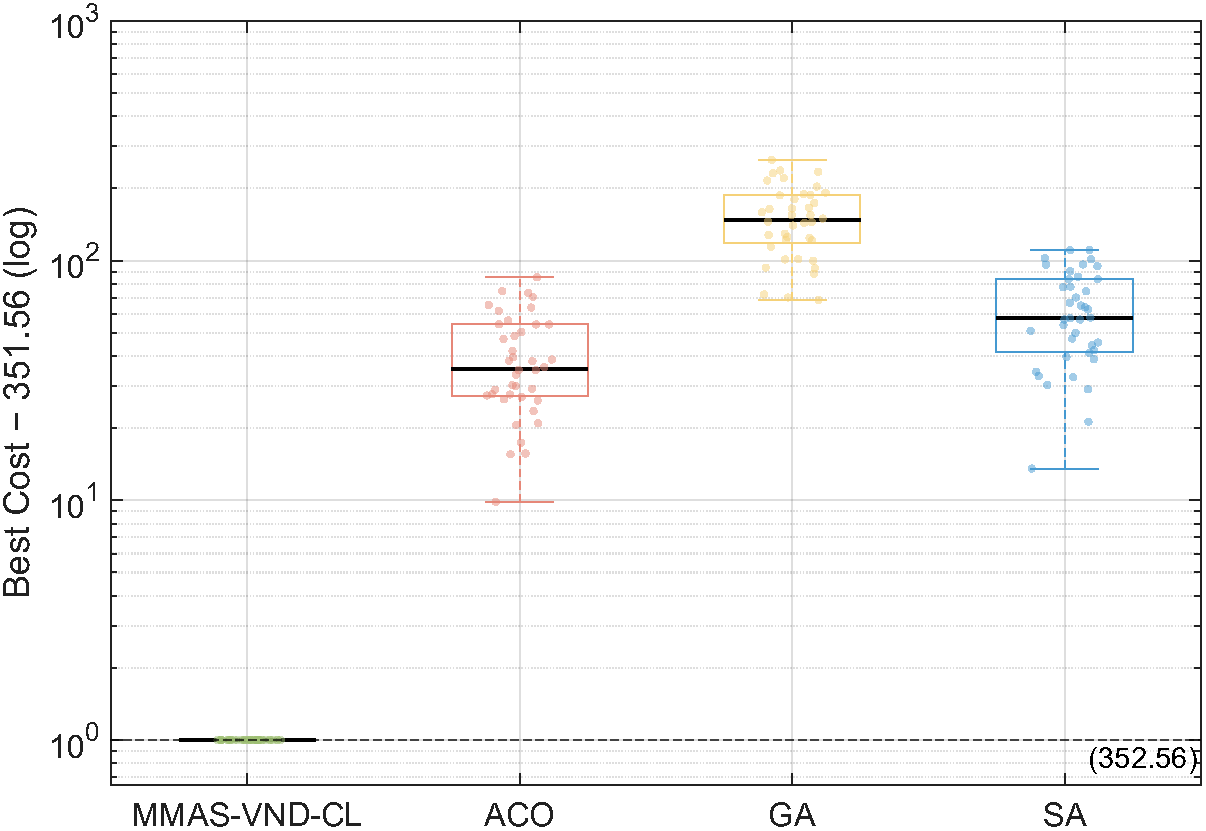
\includegraphics[width=0.3\textwidth]{figures/DifTSP_Map1_box}}\hfil
\subfloat[Map~2]{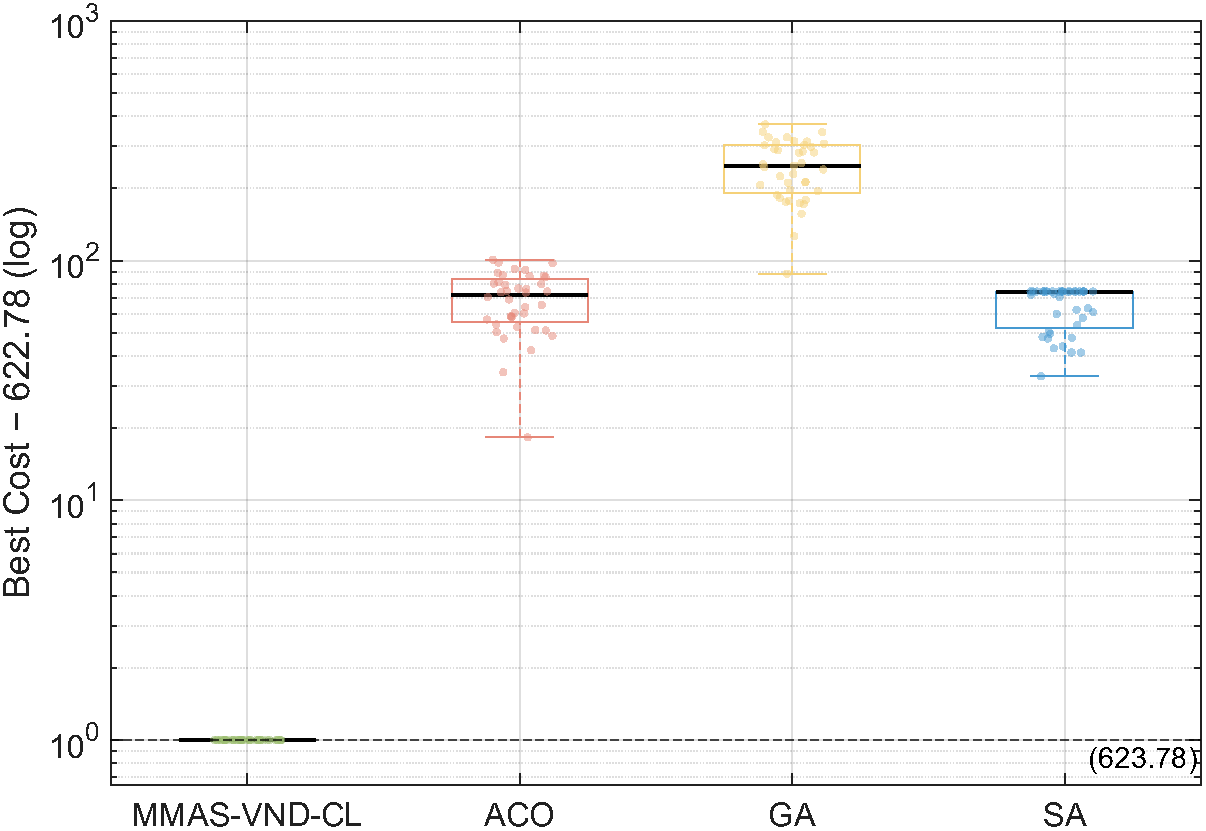
\includegraphics[width=0.3\textwidth]{figures/DifTSP_Map2_box}}\hfil
\subfloat[kroB100]{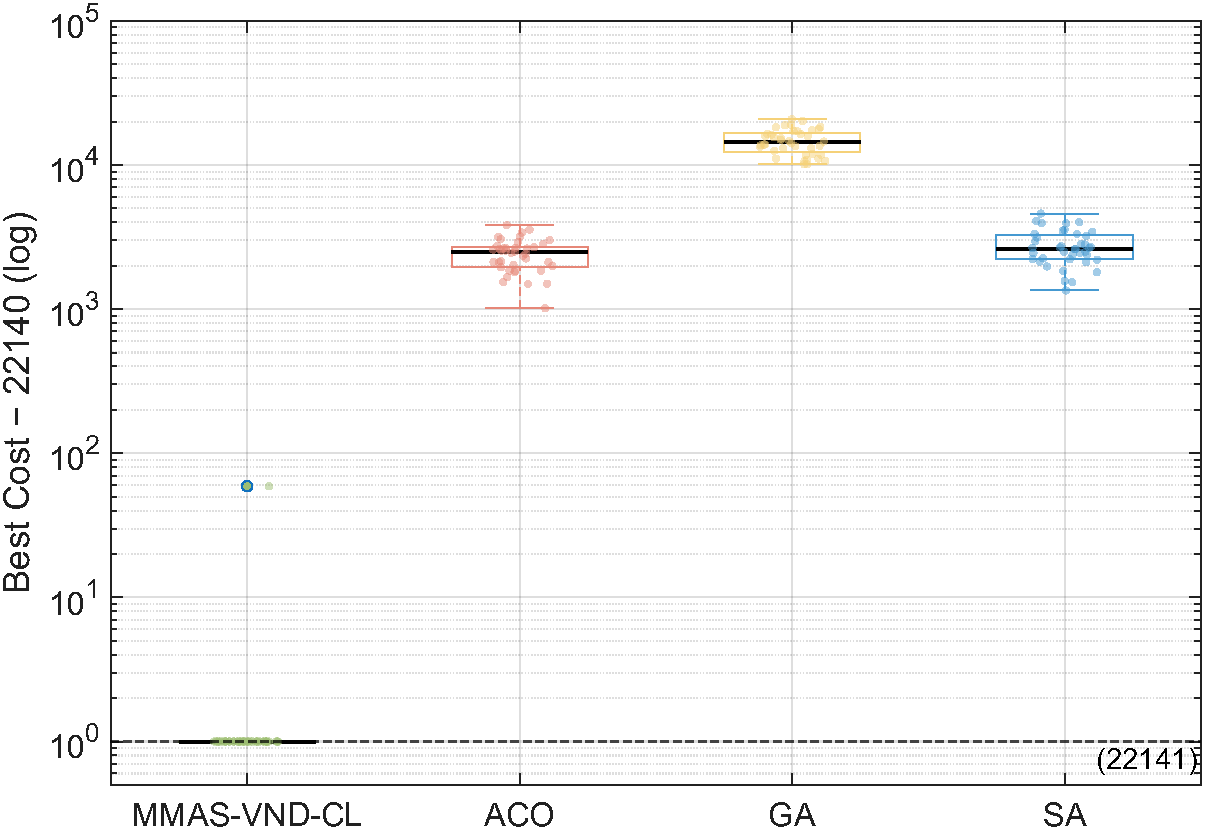
\includegraphics[width=0.3\textwidth]{figures/DifTSP_kroB100_box}}
\caption{Cost distributions of the four TSP solvers over 40 runs on the three maps.}
\label{fig:tsp_box}
\end{figure*}

\begin{figure}[!htbp]
\centering
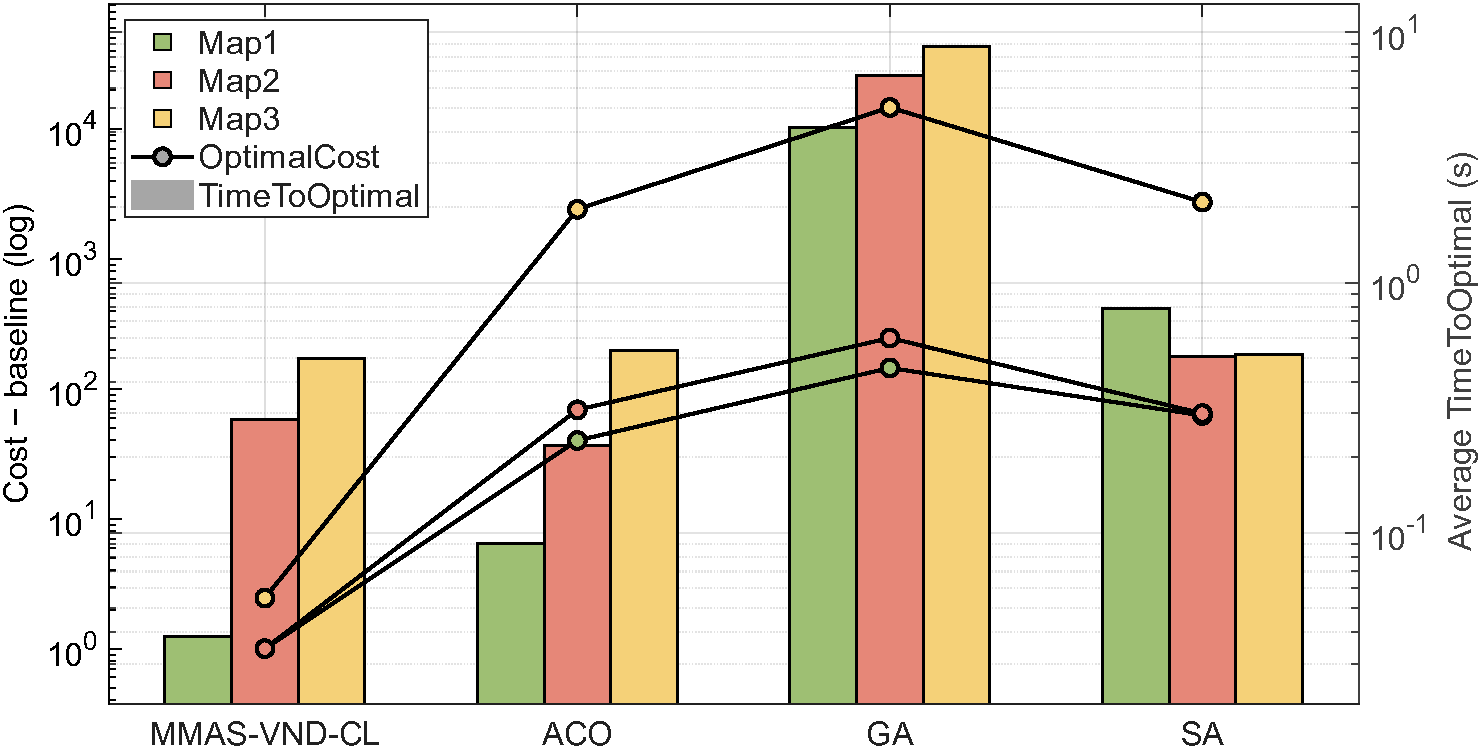
\includegraphics[width=3in]{figures/DifTSP_Map_Cost&Time}
\caption{Comparison of mean cost and mean computation time of the four TSP solvers on the three maps.}
\label{fig:tsp_cost_time}
\end{figure}

\begin{figure*}[!t]
\centering
\begin{minipage}[t]{0.48\textwidth}
\centering
\textbf{MMAS-VND-CL}\\[2pt]
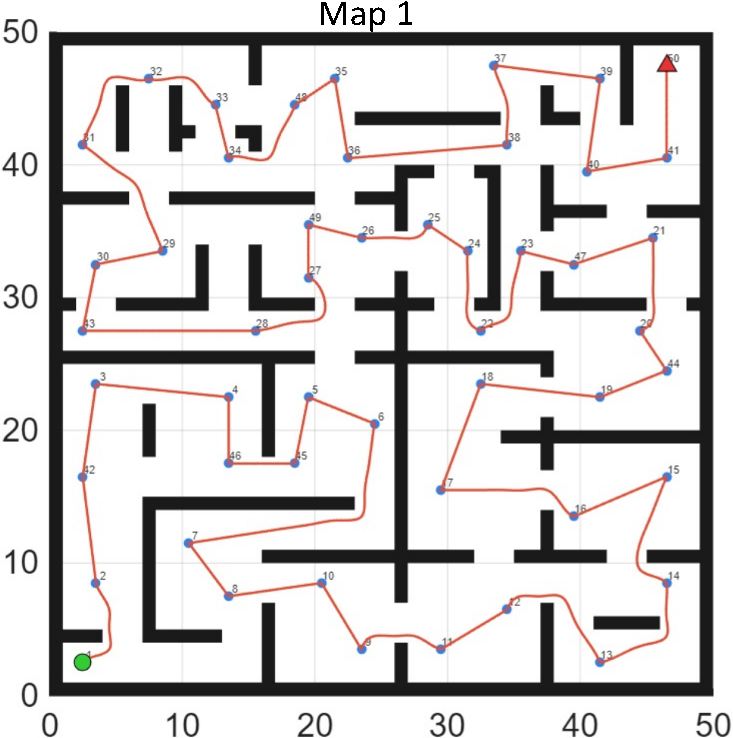
\includegraphics[width=0.46\linewidth]{figures/DifTSP_path_Map1_My}\hfil
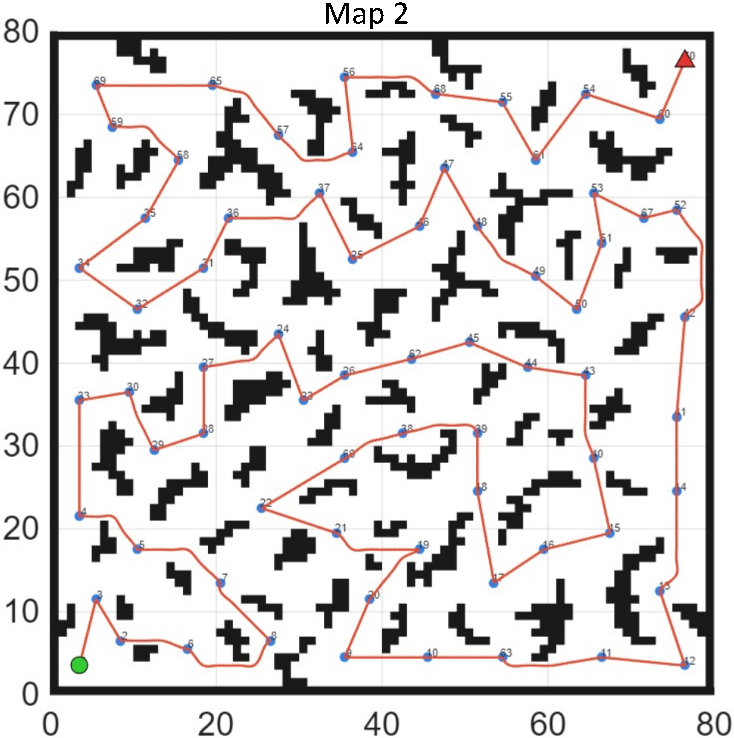
\includegraphics[width=0.46\linewidth]{figures/DifTSP_path_Map2_My}\\
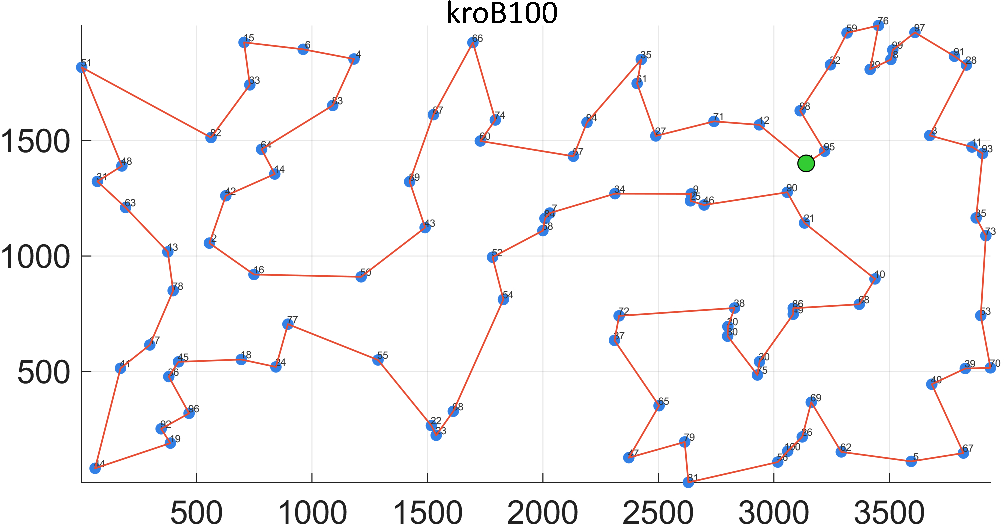
\includegraphics[width=0.78\linewidth]{figures/DifTSP_path_kroB100_My}
\end{minipage}\hfill
\begin{minipage}[t]{0.48\textwidth}
\centering
\textbf{ACO}\\[2pt]
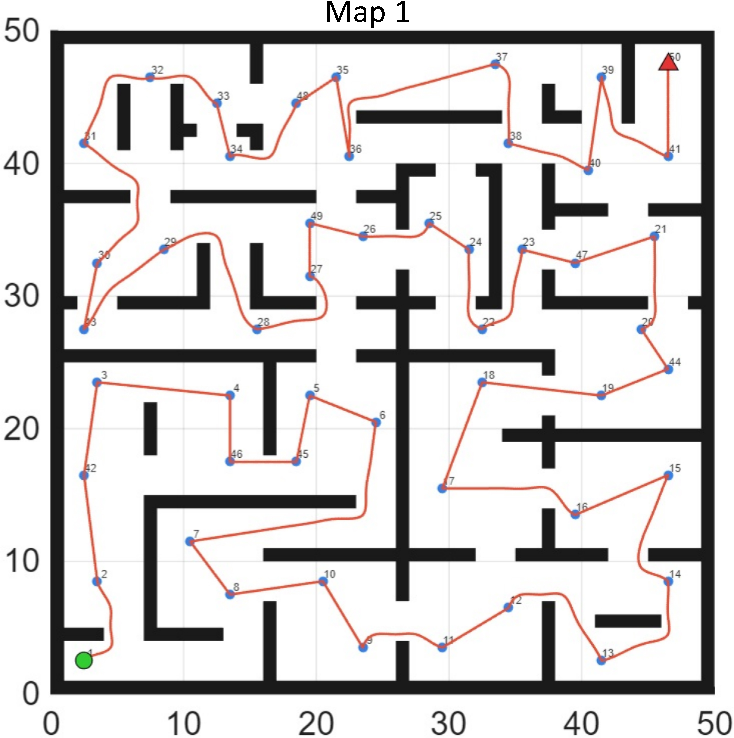
\includegraphics[width=0.46\linewidth]{figures/DifTSP_path_Map1_ACO}\hfil
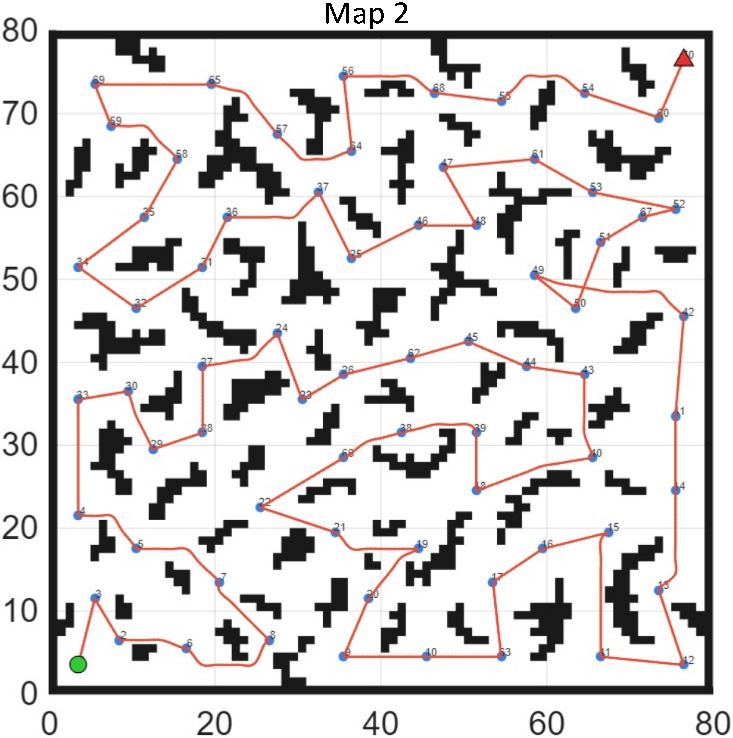
\includegraphics[width=0.46\linewidth]{figures/DifTSP_path_Map2_ACO}\\
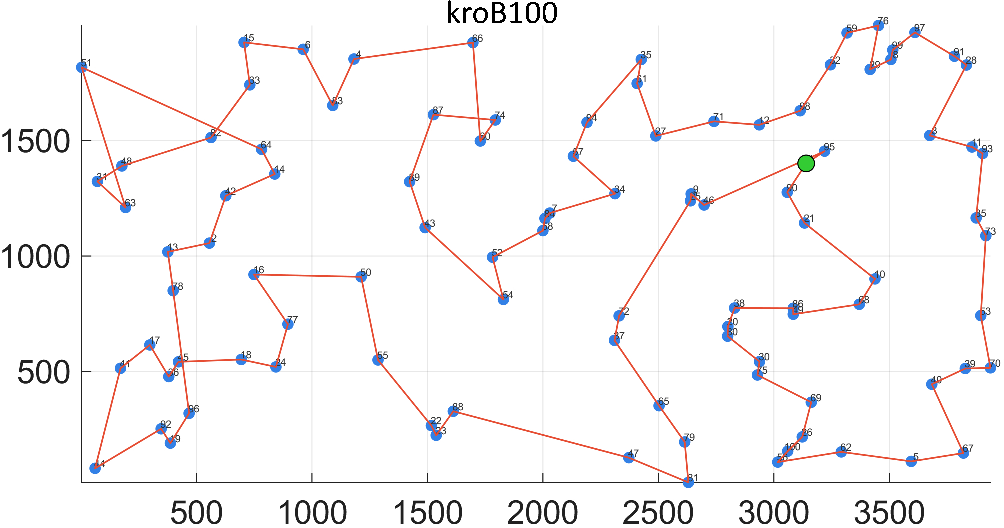
\includegraphics[width=0.78\linewidth]{figures/DifTSP_path_kroB100_ACO}
\end{minipage}

\vspace{8pt}

\begin{minipage}[t]{0.48\textwidth}
\centering
\textbf{GA}\\[2pt]
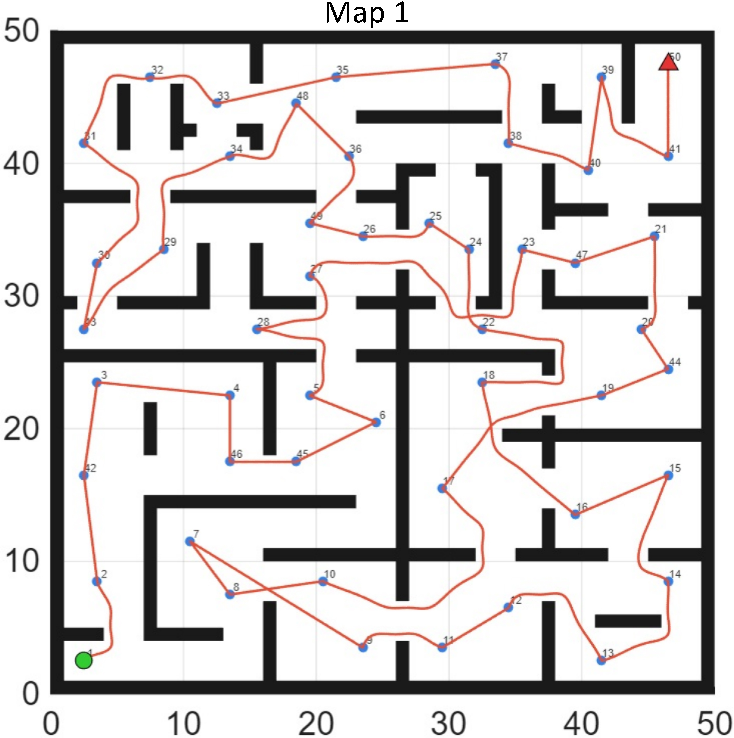
\includegraphics[width=0.46\linewidth]{figures/DifTSP_path_Map1_GA}\hfil
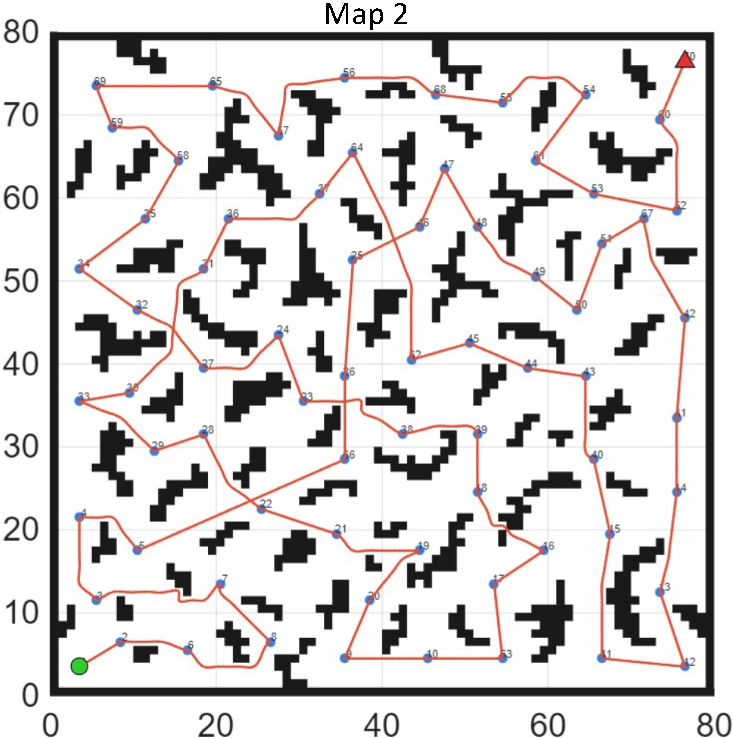
\includegraphics[width=0.46\linewidth]{figures/DifTSP_path_Map2_GA}\\
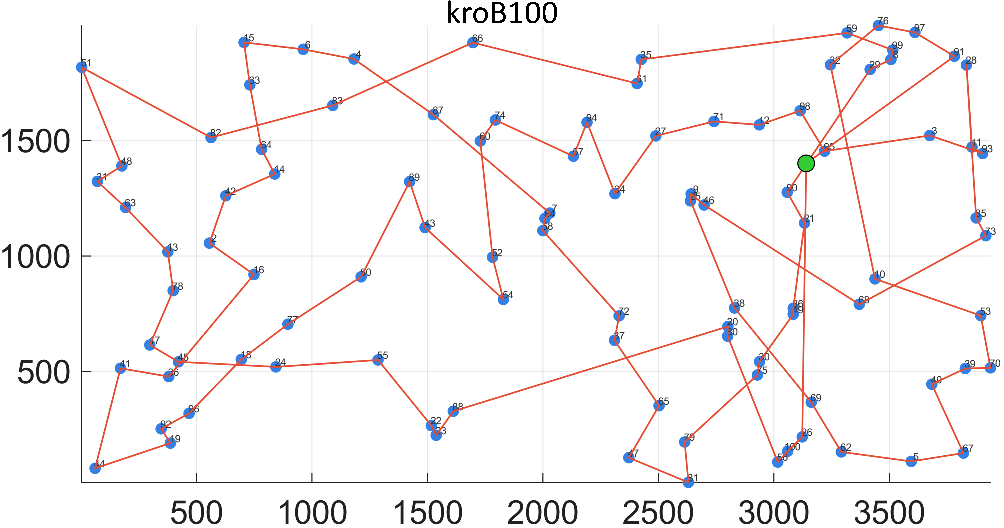
\includegraphics[width=0.78\linewidth]{figures/DifTSP_path_kroB100_GA}
\end{minipage}\hfill
\begin{minipage}[t]{0.48\textwidth}
\centering
\textbf{SA}\\[2pt]
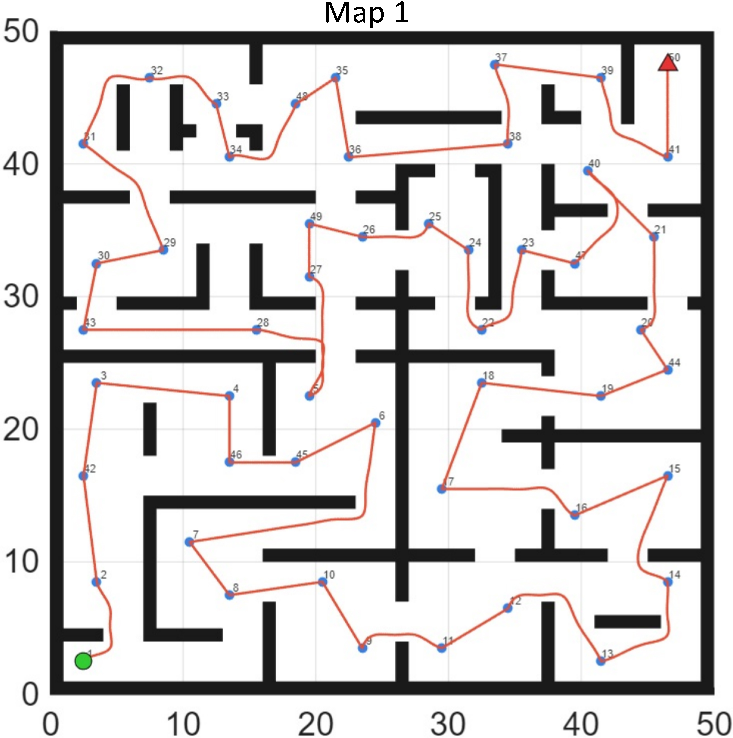
\includegraphics[width=0.46\linewidth]{figures/DifTSP_path_Map1_SA}\hfil
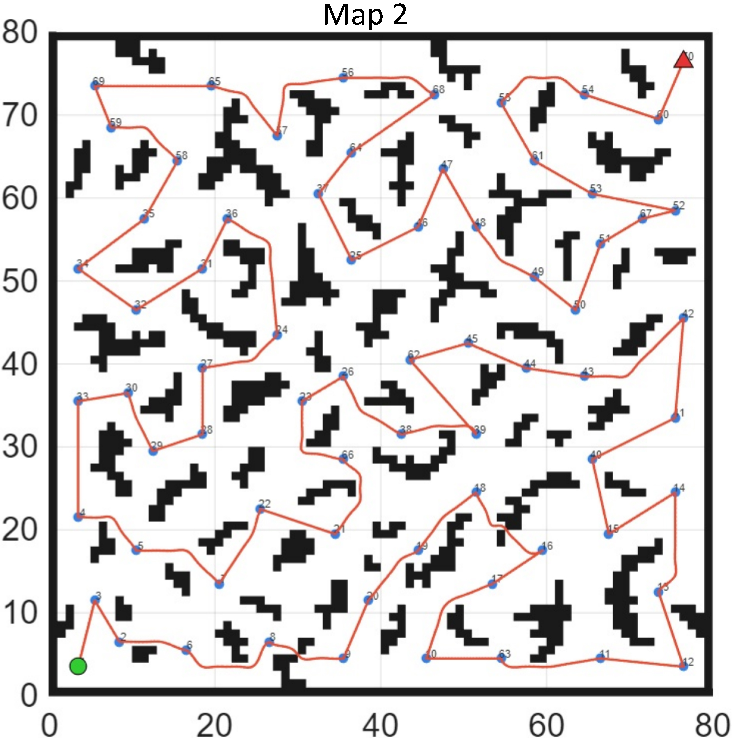
\includegraphics[width=0.46\linewidth]{figures/DifTSP_path_Map2_SA}\\
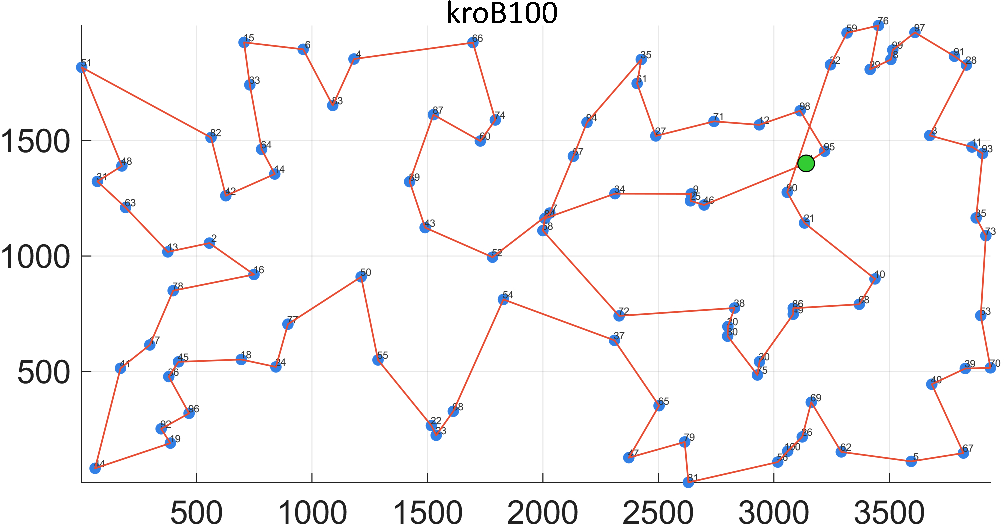
\includegraphics[width=0.78\linewidth]{figures/DifTSP_path_kroB100_SA}
\end{minipage}
\caption{Best-cost paths planned by each TSP solver on Map~1, Map~2, and kroB100.}
\label{fig:tsp_paths}
\end{figure*}

The multi-goal traversal performance of each solver is reported in Table~\textcolor{blue}{\ref{tab:tsp_cmp}}. The corresponding visualizations are shown in Figs.~\textcolor{blue}{\ref{fig:tsp_conv}}--\textcolor{blue}{\ref{fig:tsp_paths}}.

We first examine solution quality and success rate. Table~\textcolor{blue}{\ref{tab:tsp_cmp}} shows that MMAS-VND-CL attains the lowest best cost and mean cost on all three maps, and is the only solver that reliably reaches the reference optimum across repeated runs: all 40 runs reach the reference values 352.56 and 623.78 on Map~1 and Map~2, and on kroB100 the method reaches the reference value 22141 with a success rate of 97.5\% and a mean cost of 22142.45. The success rates of the other three algorithms are all 0\%, i.e., none of their 40 runs reaches the reference optimum. This does not mean that they fail to produce feasible solutions; the table shows mean costs ranging from 361.41 to 36772.55. The gap is most pronounced on kroB100: the mean cost of the compared ACO implementation is 24546.05, about 10.9\% higher than ours; SA is about 12.3\% higher; and GA, with a mean of 36772.55, is about 66\% higher. In Fig.~\textcolor{blue}{\ref{fig:tsp_paths}}, the baseline paths exhibit substantially more detours and crossings than the proposed method, and the boxes in Fig.~\textcolor{blue}{\ref{fig:tsp_box}} are longer with more dispersed whiskers, indicating that they are occasionally not too bad but systematically longer overall.

We next analyze algorithmic stability. On kroB100, the standard deviation of MMAS-VND-CL is only 9.17, whereas those of ACO, SA, and GA are 606.87, 753.20, and 2894.73, respectively, i.e., about 1.8 to 1.9 orders of magnitude smaller than ACO and SA and about 2.5 orders of magnitude smaller than GA. On Map~2, although SA has converged to 13.02, it is still higher than the zero variance of the proposed method. This can be understood from the mechanisms: the virtual-node encoding fixes the start and end nodes and includes them fully in pheromone updates; the MMAS bounds prevent early lock-in; and the candidate-list-accelerated VND performs aggressive refinement of elite tours in every generation. Together, these three factors suppress run-to-run fluctuation to a very low level. Standard ACO and SA, which lack VND and boundary control, can only rely on random perturbations during construction or neighborhood moves, so path quality scatters widely across initializations.

We then discuss time performance and offer an objective assessment with necessary concessions. In Table~\textcolor{blue}{\ref{tab:tsp_cmp}}, on Map~2 the ACO baseline is slightly faster than the proposed method, at 223.2~ms versus 241.5~ms, and is the only baseline that is superior in run time. The reason is straightforward: this baseline performs no large-scale VND neighborhood search, so each iteration is cheaper, whereas the proposed method spends part of its budget on local search and therefore has heavier iterations. On Map~1 (38.6~ms vs.\ 90.6~ms for ACO) and kroB100 (496.7~ms, faster than 516.5~ms for SA and 534.1~ms for ACO), however, the proposed method is faster: candidate-list pruning keeps the additional overhead of VND within a controllable range, whereas the baselines often require more iterations to reach comparable quality. GA falls behind on all counts: its run time on the three maps reaches several seconds while its cost remains the worst, indicating that its variable-length chromosome crossover lacks specificity for path-type representations and wastes search effort. Summarizing the time--cost trade-off in Fig.~\textcolor{blue}{\ref{fig:tsp_cost_time}}: the proposed method occupies the region of low cost and relatively low run time simultaneously, and on Map~2 it exchanges a negligible time difference for substantially better solution quality.

Finally, we provide mechanistic attribution and close the discussion. On the unified JPS cost matrix, the differences at the combination layer are isolated and amplified: the virtual-node open encoding ensures that the start and end constraints are not broken by the search; the MMAS pheromone bounds maintain diversity; ACS-style pseudo-random transfer accelerates convergence; the candidate-list VND drives the tour toward near-optimality; and the S-curve schedule together with adaptive stopping controls when and for whom refinement cost is paid. The experiments show that what truly separates the method from the baselines is the ability to reach the reference optimum reliably, rather than the best value of any single run. We also note the boundaries of the comparison conditions: the baselines use a single parameter set and a fixed iteration budget, without parameter searches comparable to those applied to the proposed method; the default parameters of the proposed method are selected by sensitivity analysis, with an iteration cap of 800 generations and additional VND local search. It should also be acknowledged that, if an application only requires a rapid feasible visit order, a lightweight ACO retains low-latency value in simple scenarios. If the number of goal points continues to grow, the computational share of VND will increase, and further strengthening of candidate-list compression or hierarchical local search will be needed. Considering quality, reliability, and computational overhead together, MMAS-VND-CL is better suited as the sequencing module for multi-goal traversal in obstacle environments under the tested configurations.

In addition to the simulated maps above, a qualitative demonstration is conducted on a grid map constructed from satellite imagery. The region is cropped from Google Maps, converted into a binary grid (black for obstacles, white for free space), and moderately refined by hand to better meet navigation requirements. From left to right, Fig.~\textcolor{blue}{\ref{fig:googlemap}} shows: the original satellite image (the red box marks the experimental site); the binarized map with the goal configuration (yellow dots for intermediate goals, the green dot for the start, and the red triangle for the destination); and the planned result overlaid on the real map background. In the demonstration, the algorithm produces continuous paths that traverse free space and connect the goals in a reasonable manner on this map. It should be emphasized that this demonstration is a qualitative display on a single binarized map, without quantitative metrics, repeated statistics, or physical experiments; its conclusion is limited to the point that the method can directly process grid environments constructed from real imagery.

\begin{figure*}[!t]
\centering
\subfloat[]{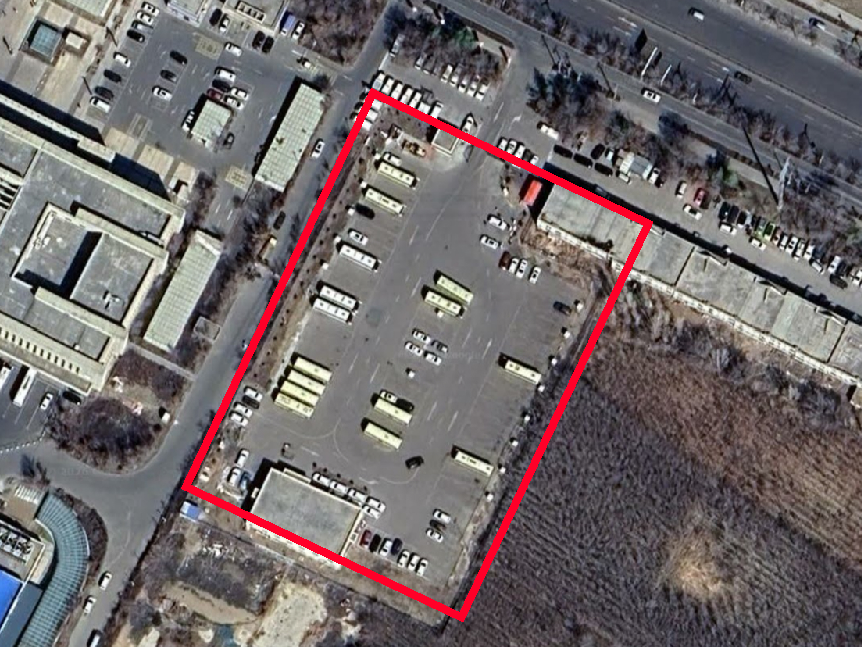
\includegraphics[height=4.2cm]{figures/GoogleMap_full}}\hfil
\subfloat[]{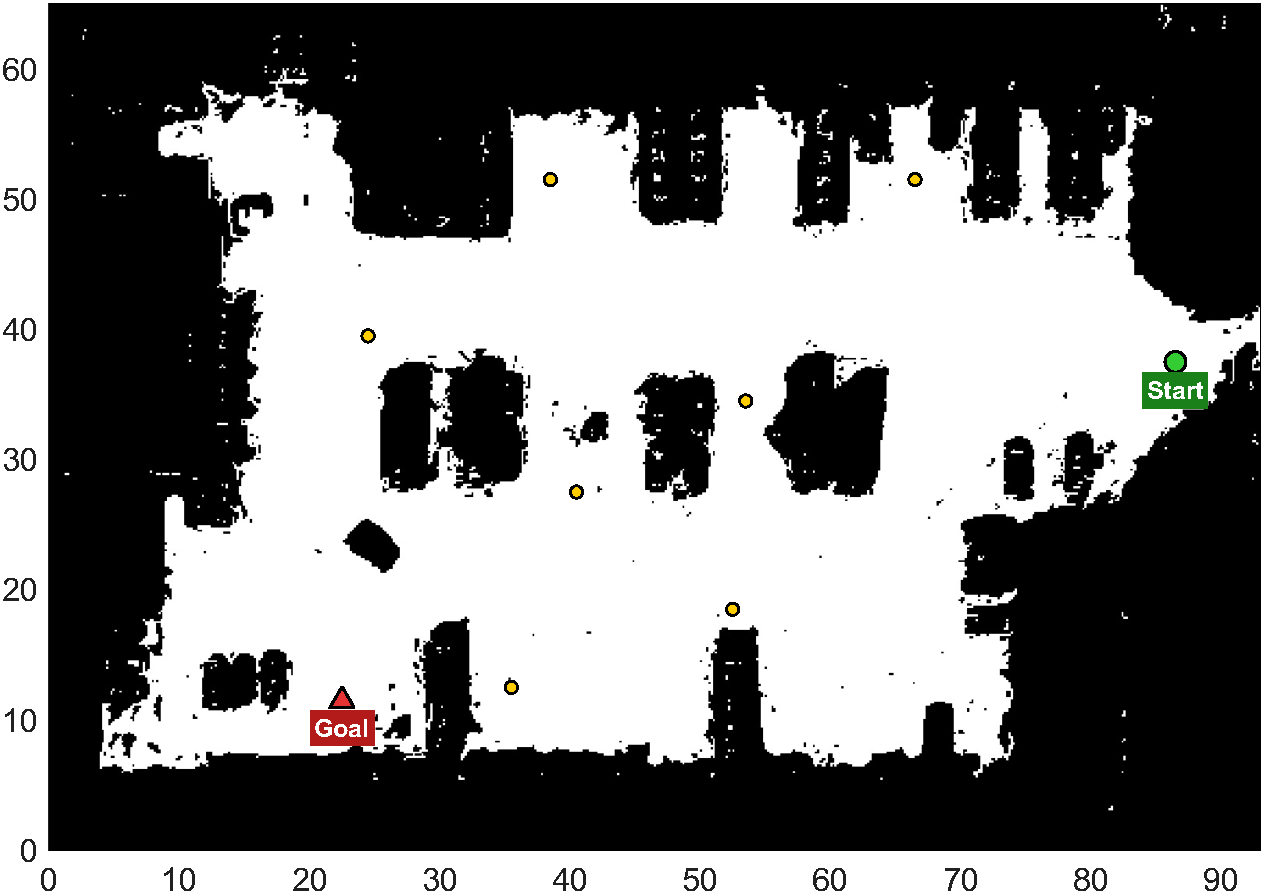
\includegraphics[height=4.2cm]{figures/GoogleMap_01goal}}\hfil
\subfloat[]{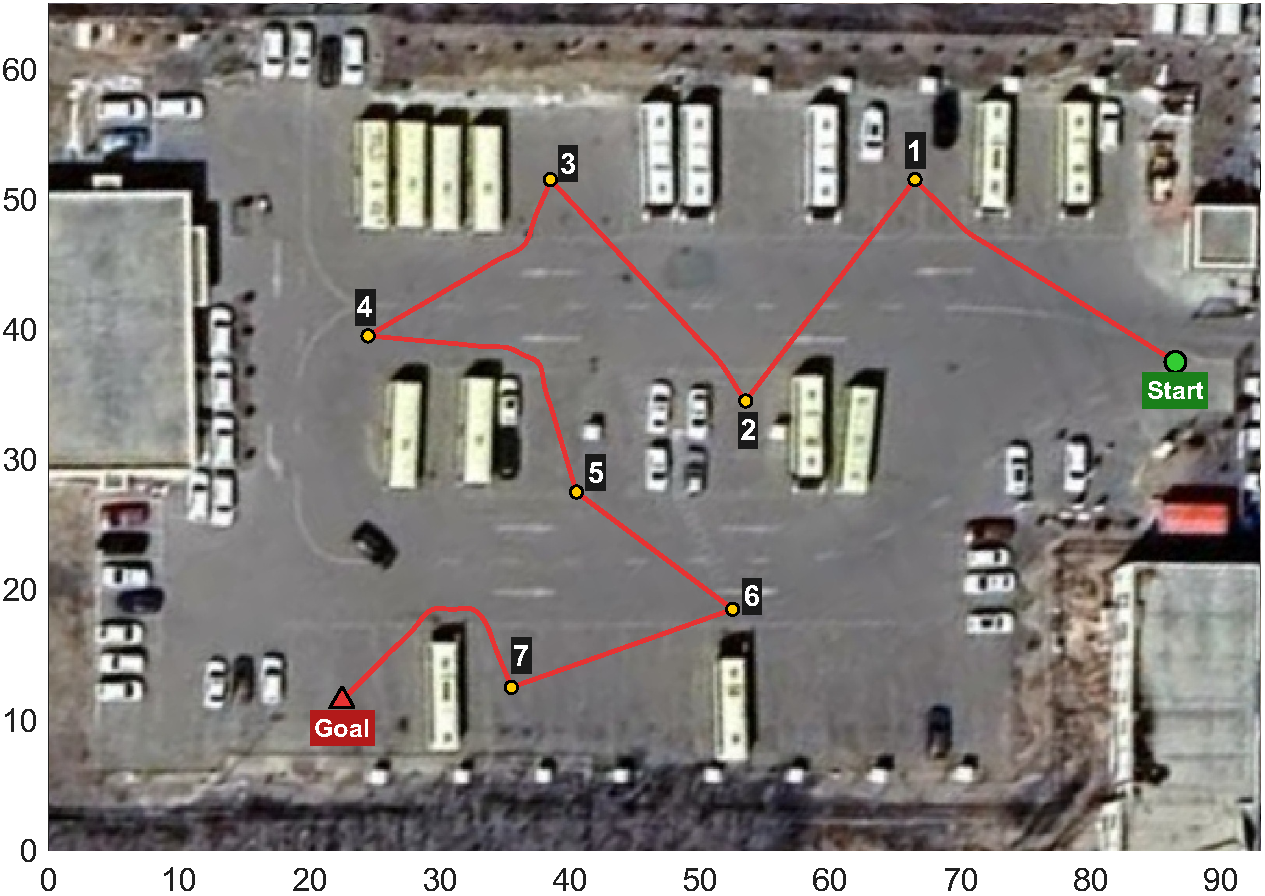
\includegraphics[height=4.2cm]{figures/GoogleMap_Path}}
\caption{Validation on a real satellite scene. (a) Region cropped from Google Maps, with the red box marking the experimental site; (b) the converted binary map and goal configuration; (c) the planned path overlaid on the real map background.}
\label{fig:googlemap}
\end{figure*}

\section{Conclusion}
\label{sec:concl}

This paper proposed a two-level planning framework for multi-goal traversal in static obstacle environments. Pairwise paths are obtained by a JPS-based improved A* search; safety-distance-aware path simplification and spline smoothing are used to construct an obstacle-constrained cost matrix from the processed continuous trajectories; and the MMAS-VND-CL solver then determines the goal visiting order. Experiments show that the improved A* achieves a planning time of 11.85 ms on Map~2, lower than conventional A* (29.19 ms) and Dijkstra (202.29 ms), and that the processed continuous trajectories are approximately 4.7\%--5.3\% shorter than the compared original grid paths. On the standard kroB100 closed-loop benchmark, MMAS-VND-CL reaches the known optimal tour cost of 22141 with a hit rate of 97.5\%, and a mean cost of 22142.45. Ablation results show that VND local search and the MMAS pheromone boundary play important roles in solution quality and stability. A grid map constructed from satellite imagery further demonstrates the method's ability to handle obstacle layouts in practical scenes.
